% =====================================================================
%  Talk version of paper/head-sets-simple.tex: one message per slide,
%  the message in the title, at most a few short bullets.
%  Same order as the paper (rules, main comparison, summed vector, beyond the
%  five templates); the coverage table is in the backup slide at the end.
%  Numbers are copied from paper/tables/{e13_main,e14_main,
%  e24_sizes_*,e26_shared,e26_task,synth_readouts}.tex; figures are paper/figures/*.pdf.
%  Compile with Tectonic from this folder:  tectonic head-sets-simple-slides.tex
% =====================================================================
\documentclass[aspectratio=169,11pt,xcolor=table]{beamer}

\usetheme{default}
\usefonttheme{professionalfonts}
\setbeamertemplate{navigation symbols}{}
\setbeamertemplate{footline}{\hfill\scriptsize\color{gray}\insertframenumber\hspace{1.2em}\vspace{0.6em}}
\setbeamertemplate{itemize items}{\textbullet}
\setbeamertemplate{itemize subitem}{\textendash}

\usepackage{booktabs,array,amsmath,amssymb}
\usepackage{fontspec}
\newfontfamily\cjkfont{FandolSong-Regular.otf}
\usepackage{tikz}
\usetikzlibrary{positioning,arrows.meta,calc,decorations.pathreplacing}
\graphicspath{{../figures/}}

% ---- colours ------------------------------------------------------------
\definecolor{ink}{HTML}{222222}
\definecolor{accent}{HTML}{1F6FB2}
\definecolor{filt}{HTML}{1AA37A}     % filter rules (green in the figures)
\definecolor{caus}{HTML}{E8693A}     % causal rules (orange in the figures)
\definecolor{soft}{HTML}{F2F4F7}
\definecolor{cBOS}{HTML}{B8B8B8}
\definecolor{cTask}{HTML}{F4B942}
\definecolor{cQuery}{HTML}{9CC3E6}
\definecolor{cMark}{HTML}{C79BD8}
\definecolor{cStop}{HTML}{CFE8C4}
\definecolor{cLast}{HTML}{F08A80}
\definecolor{acc}{HTML}{1AA37A}

\setbeamercolor{frametitle}{fg=ink}
\setbeamercolor{normal text}{fg=ink}
\setbeamercolor{structure}{fg=accent}
\setbeamerfont{frametitle}{series=\bfseries,size=\Large}

% one-line take-home message at the bottom of a slide (used sparingly)
\newcommand{\takeaway}[1]{\vfill
  \begin{beamercolorbox}[wd=\textwidth,sep=6pt]{takeaway}#1\end{beamercolorbox}}
\setbeamercolor{takeaway}{bg=soft,fg=ink}

% small grey note (sources, schematic values, how to read a figure)
\newcommand{\gnote}[1]{{\footnotesize\color{gray}#1}}

% more air between bullets
\newcommand{\spaced}{\setlength{\itemsep}{0.55em}}

% shaded accuracy cell: \cv{0.62}
\newcommand{\cv}[1]{\pgfmathtruncatemacro{\cvshade}{#1*70}\edef\cvcmd{\noexpand\cellcolor{acc!\cvshade!white}}\cvcmd#1}
\newcommand{\opt}{$^\dagger$}
\newcommand{\Causal}{\textcolor{caus}{Causal}}
\newcommand{\CausalG}{\textcolor{caus}{Causal $-$ generic}}

% a coloured token box for the prompt diagram
\newcommand{\tok}[2]{\tikz[baseline=(t.base)]\node[fill=#1,rounded corners=2pt,inner sep=2.5pt,font=\ttfamily\small](t){\strut #2};}

\title{Head Sets for Simple Tasks}
\subtitle{Which attention heads carry a task, and how to find them\\
\small Llama-3.1-8B-Instruct, 14 tasks}
\author{Filippo Merlo}
\date{November 2026}

\begin{document}

% =====================================================================
\begin{frame}
\titlepage
\end{frame}

% =====================================================================
\section{Setup}

\begin{frame}{Goal: find the few heads that carry a task}
\vspace{0.5em}
\centering
\texttt{What is the capital of the country? Q: France A:}
\quad$\rightarrow$\quad \emph{Paris}

\vspace{1.4em}
\raggedright
\begin{itemize}\spaced
\item Earlier work: the task lives in a \textbf{small set of attention heads}.
\item We want that set to be
  \begin{itemize}
  \item \textbf{small}: as few heads as possible,
  \item \textbf{general}: ideally one set for all tasks,
  \item \textbf{cheap to find}: no patching of every head.
  \end{itemize}
\end{itemize}
\end{frame}

% =====================================================================
\begin{frame}{14 simple tasks, three kinds of prompt}
\centering
\begin{tabular}{@{}lll@{}}
\toprule
Type & Tasks & Example \\
\midrule
Word relations & antonym, synonym & hot $\rightarrow$ cold \\
Morphology & singular--plural, present--past & go $\rightarrow$ went \\
Facts & capital, currency, landmark, park, product & France $\rightarrow$ Paris \\
Sequences & next-item, prev-item & Monday $\rightarrow$ Tuesday \\
Translations & English to French, German, Spanish & dog $\rightarrow$ chien \\
\bottomrule
\end{tabular}

\vspace{1.2em}
\raggedright
\begin{tabular}{@{}l@{\hspace{1em}}l@{}}
\textbf{Rule} prompt: states the task & \texttt{\footnotesize What is the capital of the country? Q: France\textbackslash nA:} \\[3pt]
\textbf{Example} prompt: shows it & \texttt{\footnotesize \ Italy: Rome; Spain: Madrid; France:} \\[3pt]
\textbf{Bare} prompt: no task & \texttt{\footnotesize \ France:} \\
\end{tabular}

\vfill
\gnote{Tasks and prompts: Yang et al.\ (2026).}
\end{frame}

% =====================================================================
\begin{frame}{How we test a set: patch the task into a bare prompt}
\centering
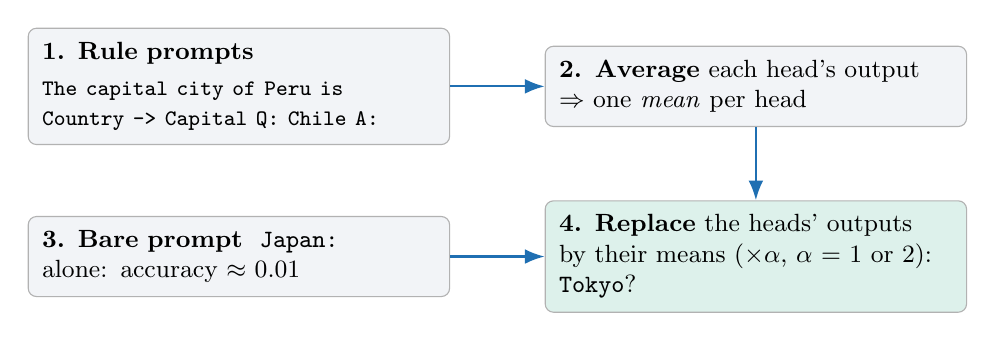
\begin{tikzpicture}[
  box/.style={draw=gray!60,rounded corners=3pt,fill=soft,align=left,font=\small,inner sep=5pt},
  arr/.style={-{Latex[length=2.5mm]},thick,accent}]
\node[box,text width=5.0cm](rule){\textbf{1. Rule prompts}\\[2pt]
  \texttt{\footnotesize The capital city of Peru is}\\
  \texttt{\footnotesize Country -> Capital Q: Chile A:}};
\node[box,text width=5.0cm,right=1.2cm of rule](mean){\textbf{2. Average} each head's output\\
  $\Rightarrow$ one \emph{mean} per head};
\node[box,text width=5.0cm,below=0.9cm of rule](bare){\textbf{3. Bare prompt} \texttt{\ Japan:}\\
  alone: accuracy $\approx$ 0.01};
\node[box,text width=5.0cm,right=1.2cm of bare,fill=acc!15](out){\textbf{4. Replace} the heads' outputs by their means ($\times\alpha$, $\alpha$ = 1 or 2): \texttt{Tokyo}?};
\draw[arr](rule)--(mean);
\draw[arr](mean)--(out);
\draw[arr](bare)--(out);
\end{tikzpicture}

\vspace{0.8em}
\raggedright
\textbf{Two checks on every set}, both should stay near zero:
\begin{itemize}
\item \textbf{Control}: same heads, a \emph{related} task's means (antonym $\leftrightarrow$ synonym).
\item \textbf{Random heads}: same number of heads per layer.
\end{itemize}
\end{frame}

% =====================================================================
\begin{frame}{Reading a head: logit lens vs.\ J-head}
\begin{columns}[c]
\column{0.52\textwidth}
\textbf{Logit lens} (``Logit-head'')\\[2pt]
Which words would the head push if its output went \emph{straight} to the output?

\vspace{1em}
\textbf{Head-JLens} (``J-head'')\\[2pt]
Which words does it push \emph{after all the layers that follow}?\\
\gnote{One linear map per head, fitted once on WikiText.}

\vspace{1em}
A head \textbf{decodes} a word if the word is in its top 10.

\column{0.44\textwidth}
\centering
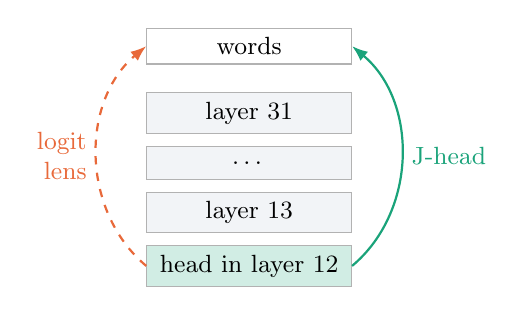
\begin{tikzpicture}[font=\small,
  lay/.style={draw=gray!60,fill=soft,minimum width=2.6cm,minimum height=0.42cm},
  arr/.style={-{Latex[length=2mm]},thick}]
\node[lay,fill=acc!20](h){head in layer 12};
\node[lay,above=0.15cm of h](l1){layer 13};
\node[lay,above=0.15cm of l1](l2){\dots};
\node[lay,above=0.15cm of l2](l3){layer 31};
\node[lay,above=0.35cm of l3,fill=white](o){words};
\draw[arr,caus,dashed](h.west)to[bend left=50]node[left,align=right]{logit\\lens}(o.west);
\draw[arr,filt](h.east)to[bend right=50]node[right,align=left]{J-head}(o.east);
\end{tikzpicture}
\end{columns}
\end{frame}

% =====================================================================
\section{Two published methods}

\begin{frame}{Method 1: lexical task heads (Yang et al., 2026)}
\centering
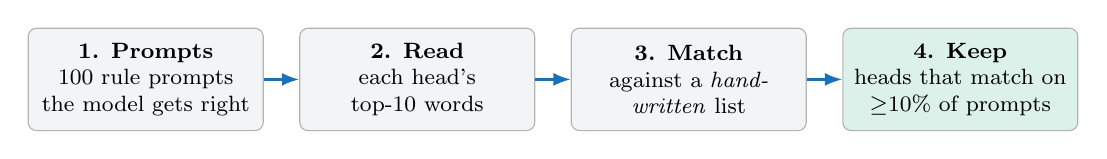
\begin{tikzpicture}[
  stp/.style={draw=gray!60,rounded corners=3pt,fill=soft,align=center,font=\footnotesize,
               text width=2.75cm,minimum height=1.3cm},
  arr/.style={-{Latex[length=2.2mm]},thick,accent}]
\node[stp](s1){\textbf{1. Prompts}\\100 rule prompts the model gets right};
\node[stp,right=0.45cm of s1](s2){\textbf{2. Read}\\each head's top-10 words};
\node[stp,right=0.45cm of s2](s3){\textbf{3. Match}\\against a \emph{hand-written} list};
\node[stp,right=0.45cm of s3,fill=acc!15](s4){\textbf{4. Keep}\\heads that match on $\geq$10\% of prompts};
\draw[arr](s1)--(s2); \draw[arr](s2)--(s3); \draw[arr](s3)--(s4);
\end{tikzpicture}

\vspace{1.2em}
\raggedright
\textbf{Example: antonym}\\[4pt]
\small
\begin{tabular}{@{}l@{\hspace{0.8em}}l@{\hspace{1em}}l@{}}
List & \tok{cTask}{opposite}\,\tok{cTask}{reverse}\,\tok{cTask}{antonym}\,\tok{cTask}{opposing}\,\tok{cTask}{{\cjkfont 反}} & \\[6pt]
Head A & \tok{cTask}{opposite}\,\tok{white}{cold}\,\tok{cTask}{reverse}\,\tok{white}{the}\,\dots & 41/100 prompts $\Rightarrow$ \textbf{kept} \\[4pt]
Head B & \tok{white}{\textbackslash n}\,\tok{white}{:}\,\tok{white}{the}\,\tok{white}{A}\,\dots & \phantom{0}3/100 prompts $\Rightarrow$ dropped \\
\end{tabular}

\vfill
\gnote{Schematic heads and counts. The set size varies by task (about 17 heads on average).}
\end{frame}

% =====================================================================
\begin{frame}{Lexical heads carry only some task types}
\vspace{0.5em}
\begin{itemize}\spaced
\item \textbf{Reproduced:} such heads exist for every task\\
      (counts within one head of theirs).
\item \textbf{On the bare prompt} they bring in mostly the \emph{fact} tasks;\\
      nothing on antonym, synonym, present--past, prev-item, translations.
\item \textbf{Their curves} reproduce only if the prompt already shows one example
      the model gets wrong (their released script).\\
      That is \emph{repairing} the task, not bringing it in.
\end{itemize}
\end{frame}

% =====================================================================
\begin{frame}{J-head finds more task heads than the logit lens}
\begin{columns}[c]
\column{0.5\textwidth}
\centering\small
\begin{tabular}{@{}lcc@{}}
\toprule
 & Logit-head & J-head \\
\midrule
\multicolumn{3}{@{}l}{\textit{Rule prompts}} \\
\quad heads found & 240 & 370 \\
\quad effect & 0.17 & 0.19 \\
\midrule
\multicolumn{3}{@{}l}{\textit{Example prompts}} \\
\quad heads found & 141 & 237 \\
\quad effect & 0.22 & 0.32 \\
\bottomrule
\end{tabular}

\vspace{0.4em}
\gnote{Heads: sum over tasks. Effect: best accuracy gain\\ on the bare prompt, mean of 14 tasks (Yang et al.'s rule).}

\column{0.46\textwidth}
\begin{itemize}\spaced
\item \textbf{50--70\% more} heads.
\item The extra ones sit in \textbf{layers 10--19}, where the logit lens sees little.
\item They have causal effects of their own.
\item The lead holds at \textbf{equal set size}.
\end{itemize}
\end{columns}
\takeaway{From here on, every head is read with J-head.}
\end{frame}

% =====================================================================
\begin{frame}{Method 2: causal score (Davidson et al., 2025)}
\centering
\scalebox{0.95}{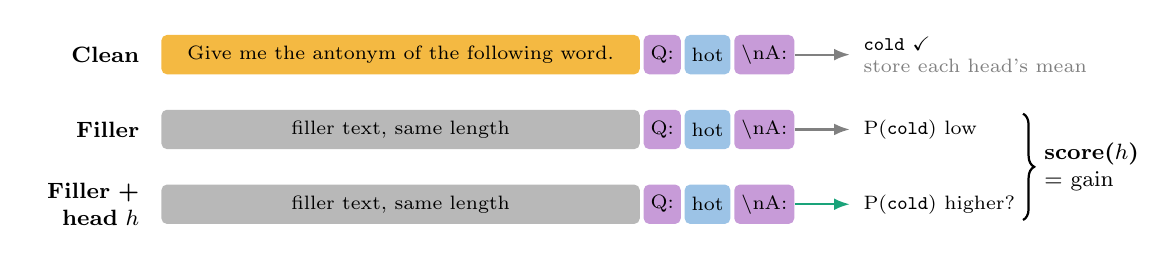
\begin{tikzpicture}[font=\scriptsize,
  lab/.style={anchor=east,align=right,text width=1.3cm,font=\footnotesize},
  tk/.style={rounded corners=2pt,minimum height=0.5cm,inner sep=2.5pt,anchor=west},
  ins/.style={tk,text width=5.9cm,align=center},
  outp/.style={anchor=west,align=left},
  arr/.style={-{Latex[length=2mm]},thick,gray}]
% row 1: clean
\node[lab] at (-0.15,0){\textbf{Clean}};
\node[ins,fill=cTask](i1) at (0,0){Give me the antonym of the following word.};
\node[tk,fill=cMark,right=1pt of i1](q1){Q:};
\node[tk,fill=cQuery,right=1pt of q1](x1){hot};
\node[tk,fill=cMark,right=1pt of x1](a1){\textbackslash nA:};
\draw[arr](a1.east)--(8.75,0);
\node[outp] at (8.8,0){\texttt{cold} \checkmark\\{\color{gray}store each head's mean}};
% row 2: filler
\node[lab] at (-0.15,-0.95){\textbf{Filler}};
\node[ins,fill=cBOS](i2) at (0,-0.95){filler text, same length};
\node[tk,fill=cMark,right=1pt of i2](q2){Q:};
\node[tk,fill=cQuery,right=1pt of q2](x2){hot};
\node[tk,fill=cMark,right=1pt of x2](a2){\textbackslash nA:};
\draw[arr](a2.east)--(8.75,-0.95);
\node[outp] at (8.8,-0.95){P(\texttt{cold}) low};
% row 3: filler + head h
\node[lab] at (-0.15,-1.9){\textbf{Filler +}\\\textbf{head $h$}};
\node[ins,fill=cBOS](i3) at (0,-1.9){filler text, same length};
\node[tk,fill=cMark,right=1pt of i3](q3){Q:};
\node[tk,fill=cQuery,right=1pt of q3](x3){hot};
\node[tk,fill=cMark,right=1pt of x3](a3){\textbackslash nA:};
\draw[arr,acc](a3.east)--(8.75,-1.9);
\node[outp] at (8.8,-1.9){P(\texttt{cold}) higher?};
\draw[decorate,decoration={brace,amplitude=4pt},thick] (10.95,-0.75)--(10.95,-2.1)
  node[midway,right=4pt,align=left,font=\footnotesize]{\textbf{score($h$)}\\= gain};
\end{tikzpicture}}

\vspace{0.8em}
\raggedright
\begin{itemize}
\item Repeat for \textbf{all 1{,}024 heads}, many prompts, three fillers; keep the top $N$.
\item \textbf{Cost:} one patched forward pass per head per prompt.
\item Theirs: \textbf{sum} the top heads' means into one vector after layer 11.\\
      Ours (\Causal\ sets): patch them \textbf{head by head}.
\end{itemize}
\vfill
\gnote{Filler: random likely tokens, WikiText text, or another task's instruction. Shared ranking: also averaged over the 14 tasks.}
\end{frame}

% =====================================================================
\begin{frame}{Generic heads: high causal score, but no task}
\vspace{0.5em}
\begin{itemize}\spaced
\item Some of the causal top 30 decode \textbf{the same tokens on every task}
      (line ends, colons): one large push shared by all tasks.
\item Dropping six of them makes Davidson et al.'s vector at least as good on all 14 tasks;
      dropping six random heads does not.
\item We mark them on the choosing half (8--9 of the top 30)\\
      and test every causal set with and without them: \CausalG.
\end{itemize}
\end{frame}

% =====================================================================
\section{Selection rules}

\begin{frame}{A fair race between rules}
\vspace{0.5em}
\begin{itemize}\spaced
\item \textbf{Same budget.} Every rule ranks all 1{,}024 heads; a set is its top $N$
      ($N$ = 20, 40, \dots, 120). Only equal sizes are compared.
\item \textbf{Two scopes.} \emph{Per task}: a set for each task.
      \emph{Shared}: one set for all 14 tasks.
\item \textbf{Held-out items.} Choose everything on one half of the items, test on the other;
      then swap and average.
\item \textbf{Scoring.} The reply must start with the full answer.
\end{itemize}
\end{frame}

% =====================================================================
\begin{frame}{Ingredient 1: a task-word list read off the heads}
\centering
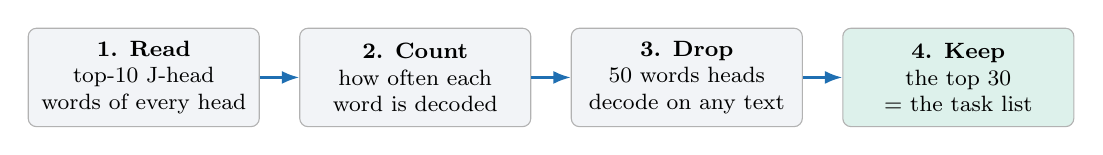
\begin{tikzpicture}[
  stp/.style={draw=gray!60,rounded corners=3pt,fill=soft,align=center,font=\footnotesize,
               text width=2.7cm,minimum height=1.25cm},
  arr/.style={-{Latex[length=2.2mm]},thick,accent}]
\node[stp](a){\textbf{1. Read}\\top-10 J-head words of every head};
\node[stp,right=0.5cm of a](b){\textbf{2. Count}\\how often each word is decoded};
\node[stp,right=0.5cm of b](c){\textbf{3. Drop}\\50 words heads decode on any text};
\node[stp,right=0.5cm of c,fill=acc!15](d){\textbf{4. Keep}\\the top 30\\= the task list};
\draw[arr](a)--(b); \draw[arr](b)--(c); \draw[arr](c)--(d);
\end{tikzpicture}

\vspace{0.8em}
\begin{columns}[T]
\column{0.5\textwidth}
\centering
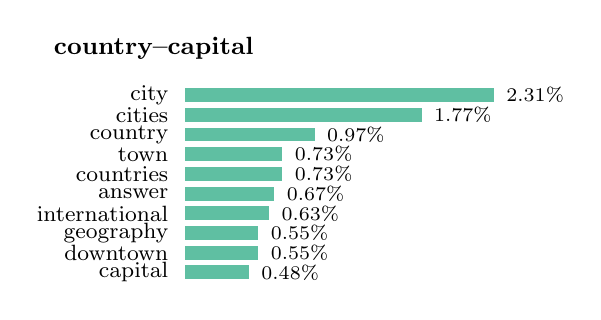
\begin{tikzpicture}[font=\footnotesize,x=1.7cm,y=-0.25cm]
\node[anchor=west,font=\small\bfseries] at (-1.0,-1.4){country--capital};
\foreach \w/\s [count=\i] in {city/2.31,cities/1.77,country/0.97,town/0.73,countries/0.73,
                              answer/0.67,international/0.63,geography/0.55,downtown/0.55,capital/0.48}{
  \node[anchor=east] at (0,\i){\w};
  \fill[acc!70] (0.05,\i-0.35) rectangle (0.05+\s,\i+0.35);
  \node[anchor=west,font=\scriptsize] at (0.07+\s,\i){\s\%};
}
\end{tikzpicture}
\column{0.46\textwidth}
\small
\textbf{antonym}\\ opposite, word, instead, because, opposing, \dots

\vspace{0.6em}
\textbf{next-item}\\ next, january, july, september, \dots

\vspace{0.6em}
\gnote{Mostly the task's own words, plus some noise\\(word pieces, numbers).}
\end{columns}
\end{frame}

% =====================================================================
\begin{frame}{Ingredient 2: where a head looks}
Attention from the last token to each \textbf{token type} (after Bai et al., 2026):

\vspace{0.8em}
\centering
\tok{cBOS}{<bos>}\,\tok{cStop}{What}\,\tok{cStop}{is}\,\tok{cStop}{the}\,\tok{cTask}{capital}\,\tok{cStop}{of}\,\tok{cStop}{the}\,\tok{cTask}{country}\,\tok{cStop}{?}\,\tok{cMark}{Q:}\,\tok{cQuery}{France}\,\tok{cMark}{\textbackslash nA}\,\tok{cLast}{:}

\vspace{1.2em}
\raggedright
Seven filters, each ranks all heads:\\[4pt]
\begin{tabular}{@{}cl@{\hspace{2.5em}}cl@{}}
\textbf{D} & decodes words of the task list & \tok{cTask}{T} & attends to the task words \\[2pt]
\tok{cBOS}{B} & attends \emph{little} to \texttt{<bos>} & \tok{cMark}{M} & attends to the Q/A markers \\[2pt]
\tok{cLast}{L} & attends to the last token & \tok{cStop}{S} & attends to punctuation, stopwords \\[2pt]
 & & \textbf{N} & attends to the whole instruction \\
\end{tabular}
\takeaway{No patching: only the lens and one forward pass per prompt.}
\end{frame}

% =====================================================================
\begin{frame}{Combining filters: average the ranks}
\begin{columns}[T]
\column{0.53\textwidth}
\textbf{1. Where each head looks}\\[4pt]
\footnotesize\setlength{\tabcolsep}{3pt}
\begin{tabular}{@{}lcccccc@{}}
 & \tok{cBOS}{BOS} & \tok{cTask}{task} & \tok{cQuery}{query} & \tok{cMark}{Q/A} & \tok{cStop}{p+s} & \tok{cLast}{last} \\[2pt]
head A & \cv{0.85} & \cv{0.02} & \cv{0.03} & \cv{0.03} & \cv{0.05} & \cv{0.02} \\
head B & \cv{0.20} & \cv{0.45} & \cv{0.10} & \cv{0.05} & \cv{0.15} & \cv{0.05} \\
head C & \cv{0.35} & \cv{0.05} & \cv{0.10} & \cv{0.30} & \cv{0.15} & \cv{0.05} \\
head D & \cv{0.40} & \cv{0.25} & \cv{0.15} & \cv{0.05} & \cv{0.10} & \cv{0.05} \\
\end{tabular}

\column{0.43\textwidth}
\textbf{2. Rank on each filter, average}\\[4pt]
\footnotesize
\begin{tabular}{@{}lccc|c@{}}
 & D & B & T & DBT \\
\midrule
head A & 2 & 4 & 4 & 3.33 \\
head B & 1 & 1 & 1 & \textbf{1.00} \\
head C & 4 & 2 & 3 & 3.00 \\
head D & 3 & 3 & 2 & \textbf{2.67} \\
\end{tabular}

\vspace{0.8em}
\normalsize\textbf{3. Keep the top $N$}\\[2pt]
\footnotesize DBT, $N=2$: \textbf{heads B and D}.
\end{columns}

\vspace{1em}
\small
Head A decodes task words well but looks only at \texttt{<bos>}: its average rank keeps it out.\\[2pt]
Shared set: each filter's ranks are first averaged over the 14 tasks.

\vfill
\gnote{Schematic: four heads, made-up values. Rank 1 = best; B ranks \emph{low} BOS attention best.}
\end{frame}

% =====================================================================
\begin{frame}{The contenders}
\begin{columns}[T]
\column{0.5\textwidth}
\textbf{Filter combinations}
\begin{itemize}\spaced
\item \textbf{Fixed in advance:} D, B, T and their combinations, DBT included.
\item \textbf{Exploratory\opt:} best of all 79 combinations.\\
      Per task: DBMN, DBTMS.\\ Shared: DBTLS, DBTMS.
\end{itemize}

\column{0.46\textwidth}
\textbf{References}
\begin{itemize}\spaced
\item \Causal: Davidson et al.'s score, head by head, with and without generic heads.
\item \textbf{Yang terms}: their hand-written list.
\item \textbf{Random} heads.
\end{itemize}
\end{columns}
\takeaway{\opt\ Picked on the same held-out accuracy we report: optimistic, still need a fresh test.}
\end{frame}

% =====================================================================
\section{Main comparison}

\begin{frame}{The big picture: accuracy vs.\ set size}
\centering
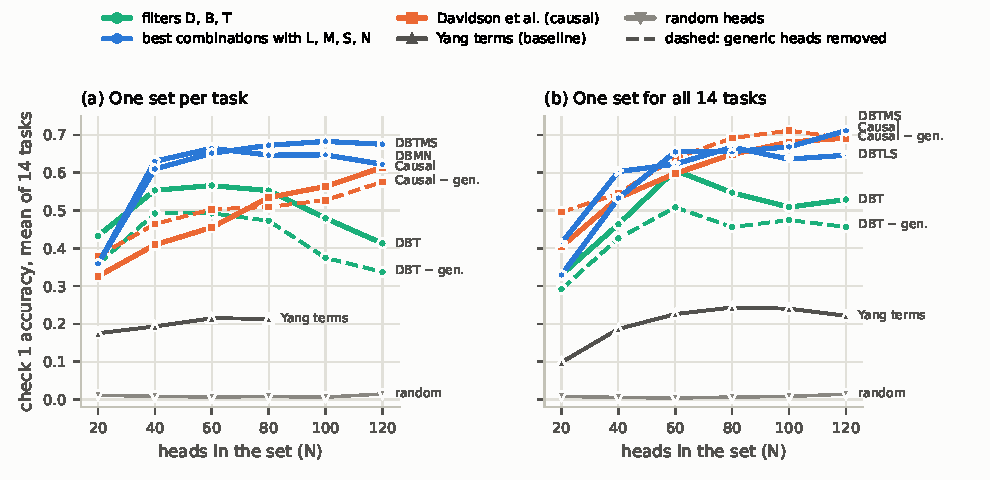
\includegraphics[height=0.74\textheight]{e13_size}

\gnote{Bare prompt, held-out items, mean of 14 tasks; no patching: 0.01. Top: fixed in advance. Bottom: exploratory\opt.}
\end{frame}

% =====================================================================
\begin{frame}{One set per task: filters match or beat the causal score}
\begin{columns}[c]
\column{0.42\textwidth}
\centering
\begin{tabular}{@{}lcc@{}}
\toprule
Per task & 40 & 80 \\
\midrule
DBT & \cv{0.55} & \cv{0.55} \\
BT & \cv{0.54} & \cv{0.55} \\
\CausalG & \cv{0.46} & \cv{0.51} \\
\Causal & \cv{0.41} & \cv{0.53} \\
Yang terms & \cv{0.19} & \cv{0.21} \\
Random & \cv{0.01} & \cv{0.01} \\
\midrule
DBMN\opt & \cv{0.63} & \cv{0.65} \\
\bottomrule
\end{tabular}

\vspace{0.3em}
\gnote{Columns: heads in the set.}

\column{0.54\textwidth}
\begin{itemize}\spaced
\item DBT and BT lead the causal score from 20 to 60 heads, level at 80.
\item They are \textbf{done by 40 heads}; the causal score keeps rising.
\item Hand-written lists stay far below.
\item Control means: $\leq$0.04.
\end{itemize}
\end{columns}
\takeaway{Per task, \emph{what a head decodes} plus \emph{where it looks} finds the task heads, with no patching.}
\end{frame}

% =====================================================================
\begin{frame}{One set for all tasks: the causal score wins}
\begin{columns}[c]
\column{0.42\textwidth}
\centering
\begin{tabular}{@{}lcc@{}}
\toprule
Shared & 40 & 80 \\
\midrule
\CausalG & \cv{0.55} & \cv{0.69} \\
\Causal & \cv{0.53} & \cv{0.65} \\
DBT & \cv{0.46} & \cv{0.55} \\
BT & \cv{0.45} & \cv{0.56} \\
Yang terms & \cv{0.19} & \cv{0.24} \\
Random & \cv{0.01} & \cv{0.01} \\
\midrule
DBMN\opt & \cv{0.58} & \cv{0.70} \\
\bottomrule
\end{tabular}

\vspace{0.3em}
\gnote{Columns: heads in the set.}

\column{0.54\textwidth}
\begin{itemize}\spaced
\item \CausalG\ is best at nearly every size (0.71 at 100 heads).
\item DBT and BT stay below it.
\item The explored filters\opt\ come level, but were picked on the test items.
\end{itemize}
\end{columns}
\takeaway{The causal score works better shared; the filters work better per task.}
\end{frame}

% =====================================================================
\begin{frame}{No rule wins every task type}
\centering
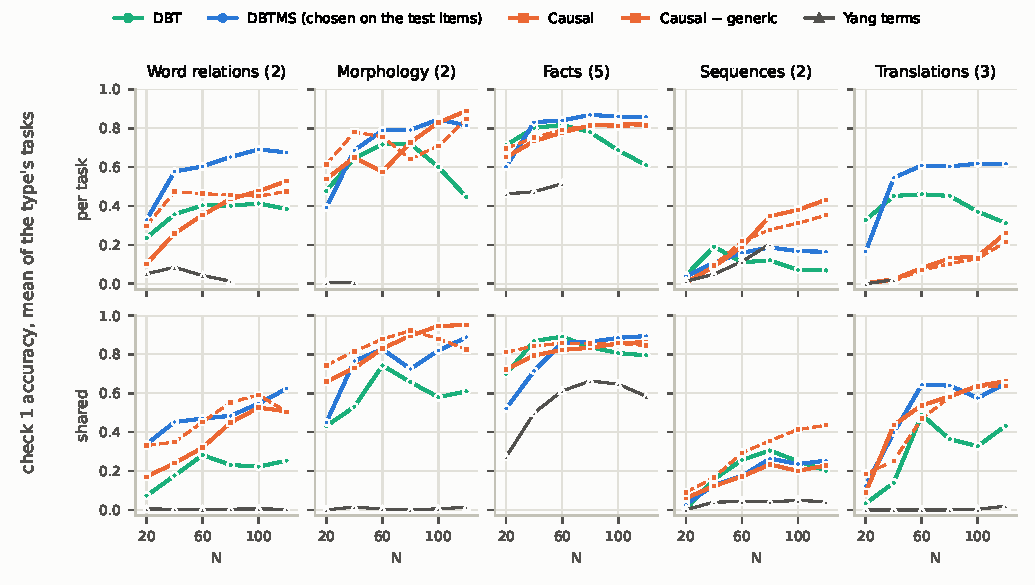
\includegraphics[height=0.6\textheight]{e13_types}

\raggedright
\begin{itemize}
\item \textbf{Facts}: almost any rule. \textbf{Sequences}: no rule.
\item \textbf{Translations}: per-task filters or a shared causal set.
      \textbf{Morphology}: causal sets and the best filters.
\end{itemize}
\end{frame}

% =====================================================================
\begin{frame}{What each filter adds (40 heads)}
\centering
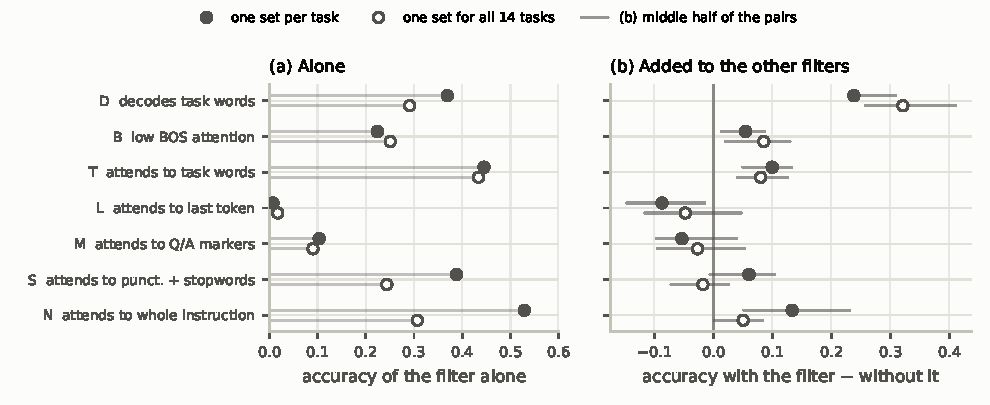
\includegraphics[width=0.9\textwidth]{e22_filters}

\raggedright
\begin{itemize}
\item \textbf{Alone}: attention to the instruction ranks best (N per task, T shared).
\item \textbf{Added to others}: decoding (D) adds most.
\end{itemize}
\takeaway{Good task heads both \emph{look at} the instruction and \emph{say} task words.}
\end{frame}

% =====================================================================
\begin{frame}{Removing generic heads helps causal sets, not filter sets}
\vspace{0.5em}
\centering
\begin{tabular}{@{}lcc@{}}
\toprule
 & with generic heads & without \\
\midrule
Shared \Causal, 20 heads & \cv{0.40} & \cv{0.50} \\
Per-task \Causal, 40 heads & \cv{0.41} & \cv{0.46} \\
Per-task DBT, 40 heads & \cv{0.55} & \cv{0.49} \\
\bottomrule
\end{tabular}

\vspace{1.2em}
\raggedright
\begin{itemize}\spaced
\item Causal sets: removing them helps in both scopes, at nearly every size.
\item DBT holds only 2--5 of them, and removing those costs accuracy.
\end{itemize}
\end{frame}

% =====================================================================
\section{Summed vector}

\begin{frame}{Summing the means into one vector loses accuracy}
Davidson et al.\ add the heads' means as \textbf{one vector} after layer 11.
Same sets, same means, both ways:

\vspace{0.6em}
\centering
\begin{tabular}{@{}llccc@{}}
\toprule
Set & & 20 heads & 40 heads & 80 heads \\
\midrule
Shared \CausalG & head by head & \cv{0.50} & \cv{0.55} & \cv{0.69} \\
 & summed & \cv{0.45} & \cv{0.46} & \cv{0.44} \\
\midrule
Shared \Causal & head by head & \cv{0.40} & \cv{0.53} & \cv{0.65} \\
 & summed & \cv{0.19} & \cv{0.38} & \cv{0.37} \\
\midrule
Per-task DBT & head by head & \cv{0.43} & \cv{0.55} & \cv{0.55} \\
 & summed & \cv{0.36} & \cv{0.43} & \cv{0.46} \\
\bottomrule
\end{tabular}

\raggedright
\vspace{0.6em}
\small The loss grows with set size, and is largest with generic heads in the set.
\takeaway{Patch head by head. For one vector: Shared \CausalG\ at 20 heads.}
\end{frame}

% =====================================================================
\section{Beyond the five templates}

\begin{frame}{Beyond the five templates}
So far: every set chosen and tested on Yang et al.'s \textbf{five rule templates}.

\vspace{0.8em}
\textbf{Two new kinds of prompt}
\begin{itemize}
\item \textbf{30 other wordings} of each task,
\item \textbf{example prompts} (5 shots): show the task instead of stating it.
\end{itemize}

\vspace{0.8em}
\textbf{Three questions}
\begin{enumerate}
\item \textbf{Transfer:} do the sets still work with the new prompts' means?
\item \textbf{Re-choosing:} do the rules, run on the new prompts, give better sets?
\item \textbf{Overlap:} how many heads do the two choices share?
\end{enumerate}
\end{frame}

% =====================================================================
\begin{frame}{Other wordings: re-choosing the heads wins back the loss}
\gnote{30 new templates per task, e.g.\\ \texttt{An antonym for \{x\} would be}\quad \texttt{Country: \{x\}\textbackslash nCapital city:}}

\vspace{0.6em}
\centering
\begin{tabular}{@{}lccc@{}}
\toprule
 & Yang's 5 & Transfer & Re-chosen \\
\midrule
Per-task DBT, 40 & \cv{0.55} & \cv{0.50} & \cv{0.57} \\
Per-task \CausalG, 40 & \cv{0.46} & \cv{0.40} & \cv{0.49} \\
Shared DBT, 80 & \cv{0.55} & \cv{0.49} & \cv{0.57} \\
Shared \CausalG, 80 & \cv{0.69} & \cv{0.61} & \cv{0.63} \\
\bottomrule
\end{tabular}

\vspace{0.3em}
\gnote{Transfer: heads from Yang's 5, means from all 35 wordings. Re-chosen: heads and means from all 35.}

\raggedright
\vspace{0.4em}
\begin{itemize}
\item New wordings cost every set some accuracy; the order of the rules stays.
\item About 3/4 of the DBT heads survive re-choosing; the causal sets change more.
\end{itemize}
\end{frame}

% =====================================================================
\begin{frame}{Example prompts: rule-chosen heads carry them, less well}
Heads chosen on \textbf{rule} prompts, patched with \textbf{5-shot example} means.

\vspace{0.4em}
\centering
\begin{tabular}{@{}llcc@{}}
\toprule
 & Set & rule means & example means \\
\midrule
Per task, 100 & DBTMS\opt & \cv{0.68} & \cv{0.64} \\
 & \Causal & \cv{0.56} & \cv{0.44} \\
 & Random & \cv{0.02} & \cv{0.03} \\
\midrule
Shared, 100 & \CausalG & \cv{0.71} & \cv{0.50} \\
 & \Causal & \cv{0.68} & \cv{0.59} \\
\bottomrule
\end{tabular}

\raggedright
\vspace{0.6em}
\begin{itemize}
\item Accuracy kept: about half at 20 heads, four fifths from 60 on.
\item Shared, the causal set does better \emph{with} its generic heads.
\item Caution: random heads from the crowded layers 11--15 reach 0.33 here.
\end{itemize}
\end{frame}

% =====================================================================
\begin{frame}{Example prompts: build the set on examples}
\begin{columns}[c]
\column{0.6\textwidth}
\centering
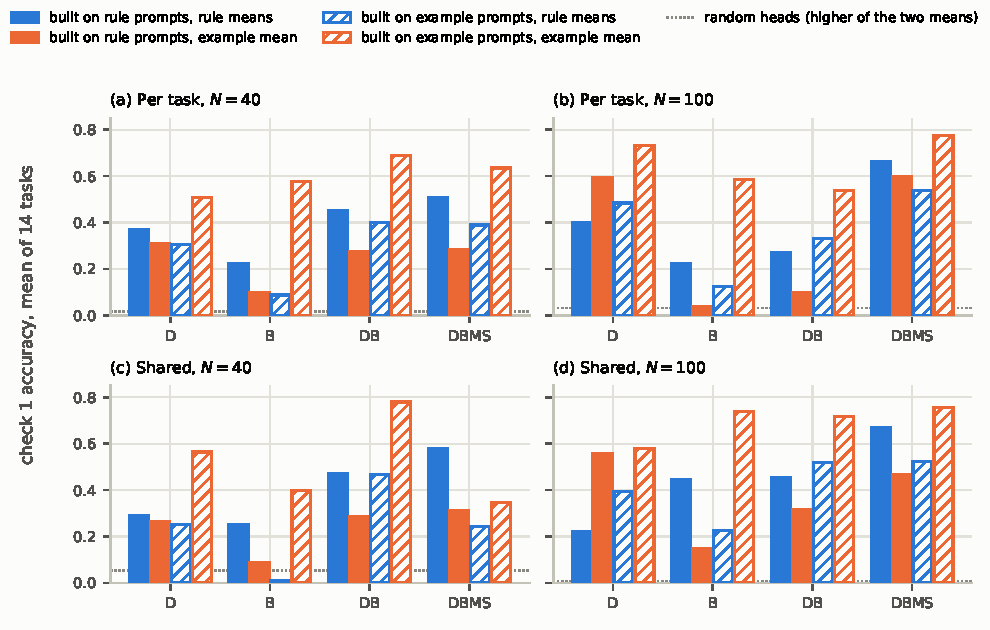
\includegraphics[width=\textwidth]{e24_grid}
\column{0.37\textwidth}
\gnote{Hatched: built on 5-shot prompts. Filled: built on rule prompts. Blue: rule means. Orange: example means.}

\vspace{0.8em}
\begin{itemize}\spaced
\item Each set works best with the means of the style it was built on.
\item Decoding heads chosen on examples also carry stated tasks.
\end{itemize}
\end{columns}
\end{frame}

% =====================================================================
\begin{frame}{The two styles pick partly the same heads}
\begin{columns}[c]
\column{0.56\textwidth}
\centering
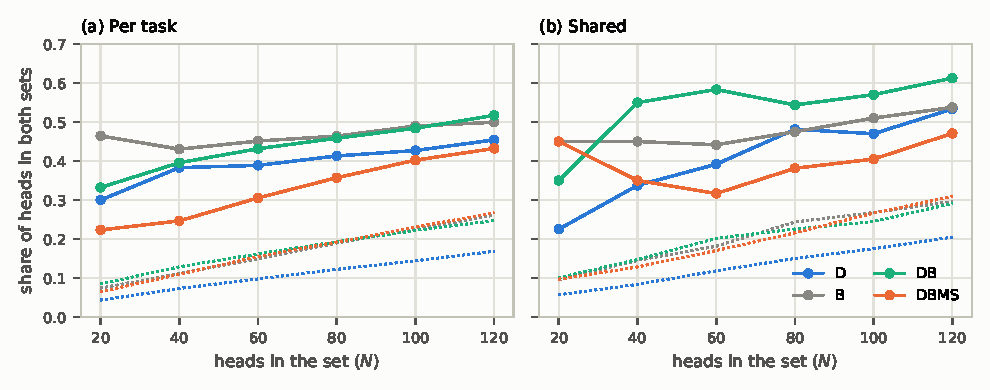
\includegraphics[width=\textwidth]{e24_overlap}

\gnote{Share of heads in both the rule-built and the example-built set. Dotted: chance.}
\column{0.4\textwidth}
\begin{itemize}\spaced
\item \textbf{2--7$\times$ chance} up to 40 heads, but \textbf{under half} the set at most sizes.
\item Marker attention (DBMS) shares least: ``\texttt{Q:}'' and ``\texttt{;}'' are different tokens.
\end{itemize}
\end{columns}
\end{frame}

% =====================================================================
\section{Conclusions}

\begin{frame}{Recipe: how to find a task head set}
\begin{enumerate}\spaced
\item \textbf{Read heads with J-head}, not the logit lens.
\item \textbf{One set per task:} rank by D, B and attention to the instruction (T, or N + M\opt).
      40--60 heads, no patching.
\item \textbf{One set for all tasks:} causal score averaged over tasks, \textbf{minus generic heads}.
      80--100 heads.
\item \textbf{Choose on the prompts the set will serve}: many wordings; examples for example tasks.
\item \textbf{Patch head by head}, not as one summed vector.
\end{enumerate}
\end{frame}

% =====================================================================
\begin{frame}{Caveats and next steps}
\begin{columns}[T]
\column{0.48\textwidth}
\textbf{Caveats}
\begin{itemize}\spaced
\item One model, 14 simple tasks, single greedy runs: 1--2 point gaps are not established.
\item Explored combinations\opt\ were picked on the test items.
\item Only $\alpha$ = 1, 2 tried.
\item New wordings checked by script only.
\item Sequences remain unsolved.
\end{itemize}
\column{0.48\textwidth}
\textbf{Next}
\begin{itemize}\spaced
\item Test the explored combinations on fresh items.
\item Hold out wordings: choose on some, test on others.
\item Choose on rule and example prompts together.
\item Move to two-hop tasks (design ready).
\end{itemize}
\end{columns}
\end{frame}

% =====================================================================
\appendix
\section{Backup}

\begin{frame}{Backup: which sets each test covers}
\centering\small
\begin{tabular}{@{}l>{\raggedright\arraybackslash}p{7.6cm}l@{}}
\toprule
Test & Sets & Sizes \\
\midrule
Five templates, head by head & every rule & 20--120 \\
Summed vector & BT, DBT, best exploratory, Causal ($\pm$ generic), Yang terms & 20--120 \\
30 other wordings & DBT, Causal ($\pm$ generic), chosen on 5 or on all 35 templates & 40--120 \\
Example mean & Causal ($\pm$ generic), Yang terms, 17 combinations & 20--120 \\
Built on example prompts & D, B, DB, DBMS & 40, 100 \\
\bottomrule
\end{tabular}

\vspace{1em}
\raggedright
\gnote{Fixed in advance: D, B, T, DB, DT, BT, DBT at every size.
Exploratory\opt: all 79 combinations of the seven filters at 40 heads, then the 15 best at every size.}
\end{frame}

\end{document}
